\documentclass[../../../../main.tex]{subfiles}

\begin{document}

\section*{第1問}

\begin{proof}[解]
\[
\ell: x=y=z, \qquad m: \frac{x}{2}=\frac{y-1}{3}=\frac{z}{-1}
\]
$t_n,s_n\in\mathbb{R}$ として（$n\in\mathbb{N}$）
\[
P_n(t_n,t_n,t_n), \qquad Q_n(2s_n,3s_n+1,-s_n)
\]
とおける。条件から，$\overrightarrow{P_nQ_n}\perp m$，$\overrightarrow{Q_nP_{n+1}}\perp\ell$ だから，
\[
\begin{pmatrix}2s_n-t_n\\3s_n+1-t_n\\-s_n-t_n\end{pmatrix}\cdot\begin{pmatrix}2\\3\\-1\end{pmatrix}=0, \qquad
\begin{pmatrix}2s_n-t_{n+1}\\3s_n+1-t_{n+1}\\-s_n-t_{n+1}\end{pmatrix}\cdot\begin{pmatrix}1\\1\\1\end{pmatrix}=0
\]
\[
\begin{cases}
4s_n+1=3t_{n+1} \\
14s_n+3=4t_n
\end{cases}
\qquad\Longrightarrow\qquad
s_n=\frac{3t_{n+1}-1}{4}=\frac{4t_n-3}{14}
\]
$s_n$ を消して，
\[
t_{n+1}-\frac{1}{13}=\frac{8}{21}\left(t_n-\frac{1}{13}\right)
\]
\[
t_n=\left(\frac{8}{21}\right)^{n-1}\left(t_1-\frac{1}{13}\right)+\frac{1}{13} \longrightarrow \frac{1}{13} \quad (n\to\infty)
\]
\[
s_n=\frac{4t_n-3}{14} \longrightarrow \frac{4\cdot\frac{1}{13}-3}{14}=-\frac{5}{26} \quad (n\to\infty)
\]
だから
\[
P_n\to\left(\frac{1}{13},\frac{1}{13},\frac{1}{13}\right), \qquad Q_n\to\left(-\frac{5}{13},\frac{11}{26},\frac{5}{26}\right)
\]
\end{proof}

\newpage

\section*{第2問}

\begin{proof}[解]
$s=\sin x$ とおく。$f(s)=s\left(1-\dfrac a2(1-s^2)\right)$ の $\max$ が1となる $a$ の値域をもとめれば良い。$f'(s)=\dfrac32as^2+\left(-\dfrac a2+1\right)$ より，$a$ によって下表を得る。

\textbf{ア．$a\ge0$ の時}

\textbf{$1^\circ$ $-\dfrac a2+1\ge0\ \therefore\ 0\le a\le2$ の時}

$f'(s)\ge0$ から，$f(s)$ は $s=1$ で $\max\ 1$

\textbf{$2^\circ$ $1-\dfrac a2\le0\le a+1\ \therefore\ 2\le a$ の時}

\begin{center}
\begin{tabular}{c|c|c|c|c|c}
$s$ & $-1$ & $-\sqrt{\frac{a-2}{3a}}$ & & $\sqrt{\frac{a-2}{3a}}$ & $1$ \\
\hline
$f'$ & & $+$\ $0$\ $-$ & & $0$\ $+$ & \\
\hline
$f$ & & $\nearrow\ \searrow$ & & $\nearrow$ & $1$
\end{tabular}
\end{center}
（$f'(s)=0$ の時，$s^2=\dfrac{a-2}{3a}$，$\alpha=\sqrt{\dfrac{a-2}{3a}}$ とおく）
\[
f(-\alpha)=-\alpha\cdot\frac{2-a}{3}\ge0 \quad (\because 2\le a)
\]
であり，$f(-\alpha)\le1$ の時 $(\alpha+1)(\alpha-8)\le0$ で，$2\le a\le8$ の時である。 $\cdots$①

\textbf{イ．$a=0$ の時}

$f'(s)=1>0$ から，$\max f=f(1)=1$

\textbf{ウ．$a<0$ の時}（$1-\dfrac a2>0$）

\textbf{$1^\circ$ $a+1\le0\ \therefore\ a\le-1$ の時}

\begin{center}
\begin{tabular}{c|c|c|c|c|c}
$s$ & $-1$ & $-\alpha$ & & $\alpha$ & $1$ \\
\hline
$f'$ & & $-$\ $+$ & & $-$ & \\
\hline
$f$ & $-1$ & $\searrow\ \nearrow$ & & $\searrow$ &
\end{tabular}
\end{center}
\[
f(\alpha)=\alpha\cdot\frac{2-a}{3}\le1
\]
の時（①より）$a=-1$

\textbf{$2^\circ$ $a+1\ge0\ \therefore\ -1\le a<0$ の時}

$f'(s)>0$ から $s=1$ で $\max\ 1$

以上ア〜ウより，$-1\le a\le8$
\end{proof}

\newpage

\section*{第3問}

\begin{proof}[解]
$F(x)=P(x)C-Q(x)S$ とおく。（$C=\cos x, S=\sin x$）

\begin{enumerate}
  \item[(1)] 全ての $x$ に対して $F(x)=0$ となる時，$P(x)\ne0$ かつ $Q(x)\ne0$ なる $x$ に対して，
  $A=P(x)^2+Q^2(x)$ とおいて，（$A\ne0$）
  \[
  F(x)=\sqrt{A}\sin(x+\alpha) \quad \left(\alpha\text{は}\ \tan\alpha=-\frac{P(x)}{Q(x)}\ \text{をみたす}\ -\pi/2<\alpha<\pi/2\text{の数}\right)
  \]
  とかける。これが任意の $x$ で0になることはないので，$A=0$ が恒等的になり立つ。つまり恒等的に $P(x)=0,\ Q(x)=0$ である。

  \item[(2)]
  \[
  P(x)\cdot C+\int_0^xQ(t)\sin t\,dt=(x^2+2x+3)S \quad \cdots \text{①}
  \]
  $x=0$ として，
  \[
  P(0)=0 \quad \cdots \text{②}
  \]
  ①の両辺 $x$ で微分して，
  \[
  -P(x)S+P'(x)C+Q(x)\cdot S=(2x+2)S+(x^2+2x+3)C
  \]
  \[
  [Q(x)-P(x)-(2x+2)]S=(x^2+2x+3-P'(x))C
  \]
  $P,Q$ は3次以下で，(1)とあわせて
  \[
  \begin{cases}
  Q(x)-P(x)=2x+2 \\
  P'(x)=x^2+2x+3
  \end{cases}
  \quad \cdots \text{③④}
  \]
  ④の両辺積分して，②とあわせて
  \[
  P(x)=\frac13x^3+x^2+3x
  \]
  ③に代入
  \[
  Q(x)=\frac13x^3+x^2+5x+2
  \]
\end{enumerate}
\end{proof}

\newpage

\section*{第4問}

\begin{proof}[解]
$C: y=\log x$，$(\log x)'=\dfrac1x$ より，$C$ 上 $x=t$ での接線は
\[
\ell_t: y=\frac1t(x-t)+\log t
\]
だから
\[
\ell_a: y=\frac1a(x-a)+\log a, \qquad \ell_c: y=\frac1c(x-c)+\log c
\]
とおり，$\ell_a,\ell_c$ の交点 $R$ の $x$ 座標は
\[
x_R=\frac{ac(\log c-\log a)}{c-a}
\]
である。

\begin{center}
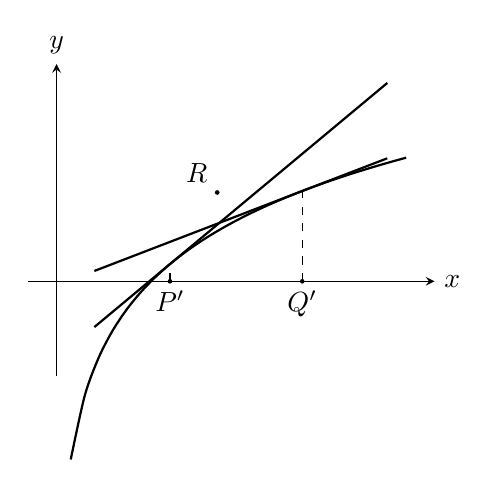
\begin{tikzpicture}[scale=1.2, >=stealth]
  \draw[->] (-0.3,0) -- (4,0) node[right] {$x$};
  \draw[->] (0,-1) -- (0,2.3) node[above] {$y$};
  \draw[domain=0.15:3.7, smooth, thick] plot (\x, {ln(\x)});
  \draw[thick, domain=0.4:3.5] plot (\x, {(\x-1.2)/1.2+ln(1.2)});
  \draw[thick, domain=0.4:3.5] plot (\x, {(\x-2.6)/2.6+ln(2.6)});
  \fill (1.7,0.94) circle (0.7pt) node[above left] {$R$};
  \fill (1.2,0) circle (0.7pt) node[below] {$P'$};
  \fill (2.6,0) circle (0.7pt) node[below] {$Q'$};
  \draw[dashed] (1.2,0) -- (1.2,{ln(1.2)});
  \draw[dashed] (2.6,0) -- (2.6,{ln(2.6)});
\end{tikzpicture}
\end{center}

\[
S=\int_a^c\log x\,dx=\left[x(\log x-1)\right]_a^c=c(\log c-1)-a(\log a-1) \quad \cdots \text{①}
\]
$P'Q'$ を底辺，$R$ の $y$ 座標を高さとする三角形として，$f(x)=x\log x$ とおくと，$T=\dfrac12(c-a)\cdot(R\text{の}y\text{座標})$ であり，接線の性質から
\[
T=\frac12\left(f(c)-f(a)\right)=\frac12(c\log c-a\log a) \quad \cdots \text{②}
\]
①②から，もとめる比は
\[
S:T=\bigl\{c(\log c-1)-a(\log a-1)\bigr\}:\frac12(c\log c-a\log a)
\]
\end{proof}

\end{document}
